
\section{Linearizzazione dei sistemi}
In mancanza della condizione di tempo invarianza può variare l'analisi del
sistema, verranno analizzati sistemi con discontinuità ma non sistemi che
variano con continuità nel tempo i loro parametri.

I sistemi non lineari sono composti da variabili e da parametri, i parametri
non sono mai forniti con un'accuratezza infinita, di conseguenza anche i
risultati in uscita avranno una certa incertezza.

Si suppone di modellare un sistema monodimensionale non lineare avendo fissato
una $\overline{u}(t)$ e si vuole mostrare l'andamento di $\dot x$ in funzione
di $x$, ricercando i vari punti di equilibrio.

%Curva di lavoro totale
\begin{figure}[h]
 \centering
 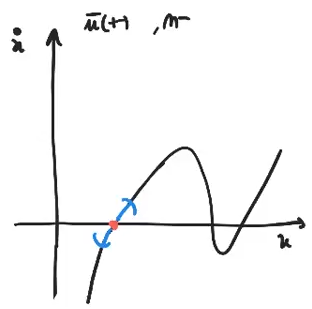
\includegraphics[width=\picwid]{curva_non_lineare.png}
 % curva_non_lineare.png: 312x309 px, 96dpi, 8.25x8.17 cm, bb=0 0 234 232
 \label{Fig.:curva_non_lineare}
\end{figure}

Si suppone che il sistema si trovi nel punto di lavoro $A$ indicato sul
grafico, nella realtà si troverà nell'intorno di quel punto oscillando in un
certo intervallo in funzione dei disturbi interni ed esterni al sistema.

Si suppone di ingrandire la curva nell'intorno del punto di lavoro

% Immagine ingrandita
\begin{figure}[h]
 \centering
 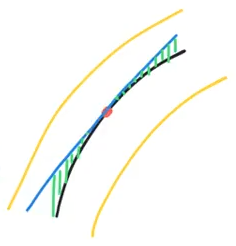
\includegraphics[width=\picwid]{curva_non_lineare_ingrandita.png}
 \label{Fig.:curva_non_lineare_ingrandita}
\end{figure}
Si considera una retta tangente alla curva nel punto di equilibrio, una retta è
sinonimo di un modello lineare, l'errore aggiuntivo commesso può ritenersi
trascurabile se minore dell'accuratezza fornita dal modello sesso.

Il vantaggio ottenuto da tale approssimazione è la possibilità di risolvere
analiticamente un sistema lineare piuttosto che cercare un teorema in grado di
risolvere quel particolare sistema non lineare.

Se si sposta di molto il punto di lavoro del sistema è necessario ricalcolare
la linearizzazione del sistema, non potendo più utilizzare la retta precedente.
Si ottiene ancora una buona approssimazione.

Ha senso linearizzare solo i punti di equilibrio, altrimenti il sistema non si
troverebbe nell'intorno di un punto, si potrebbe estendere il concetto anche a
punti di equilibrio dinamici.

$$\left\{
\begin{aligned}
\dot{x} &= f(x,u) \\
y &= g(x,u)
\end{aligned}\right.$$
Si ipotizza che le funzioni $f$ e $g$ siano sufficientemente regolari, ossia
che esista almeno il differenziale primo.

Si suppone inoltre che il sistema sottoposto ad un ingresso costante
$\overline{u}$ si trovi in un punto di equilibrio $\overline{x}$ a cui
corrisponde un'uscita di equilibrio $\overline{y}$, ossia
$$
(\overline{u},\overline{x},\overline{y}) \ \text{punto di equilibrio}
$$

Si applica la seguente posizione
$$
x(t) = \overline{x} + \delta x(t)
$$
dove $\delta x(t)$ è l'errore della traiettoria rispetto al punto di lavoro,
ovvero lo spessore definito prima nell'intorno del punto.

Analogamente per l'ingresso $u(t)$
$$
u(t) = \overline{u} + \delta u(t)
$$
Gli ingressi si suddividono in \textit{manipolabili} e \textit{non
manipolabili} dunque
anche gli ingressi sono affetti da errore e rumore,  è necessario tenere conto
di questi errori mediante
$$
y(t) = \overline{y}+\delta y(t)
$$

Tutte le precedenti equazioni sono vettoriali.

Derivando l'equazione dello stato
$$
\dot{x} = \dot{\overline{x}} + \dot{\delta x} = \dot{\delta x}
$$
quindi la variazione dello stato coincide con la variazione locale. Si può
sviluppare in serie di Taylor nel punto di equilibrio
\begin{equation}
\dot{\delta x} = \cancel{f(\overline{x},\overline{u})} + \left.\frac{\partial
f}{\partial x}\right|_{\text{eq}}\delta x + \left.\frac{\partial f}{\partial
u}\right|_{\text{eq}}\delta u + o(\delta x, \delta u)
\label{eq.:linearizzazione_sistema}
\end{equation}
La funzione di transizione valutata su un punto di equilibrio è nulla per
definizione di punto di equilibrio, il termine $\frac{\partial f}{\partial x}$
è una matrice Jacobiana con numero di righe pari al numero di righe della $f$
dunque $n$ ed un numero di colonne pari al numero di elementi della $x$, ancora
$n$ quindi è una matrice $n\times n$, la matrice verrà chiamata $A$.

Il termine $\frac{\partial f}{\partial u}$ ha invece $n$ righe ed $m$ colonne
dove $m$ è il numero di ingressi, verrà chiamata $B$.

Si riscrive la \ref{eq.:linearizzazione_sistema} trascurando l'o-piccolo si
ottiene

$$\begin{aligned}
\dot x &= \dot{\delta x} = A\delta x + B \delta u
\end{aligned}$$
quella ottenuta è proprio l'equazione di un sistema dinamico lineare con
variabile di stato pari a $\delta x$ ed ingresso pari a $\delta u$

La variazione dell'uscita invece sarà
$$\begin{aligned}
y &= \overline{y} + \delta y = g(\overline{x},\overline{u}) +
\left.\frac{\partial
g}{\partial x}\right|_{\text{eq}}\delta x + \left.\frac{\partial g}{\partial
u}\right|_{\text{eq}}\delta u + o(\delta x, \delta u) \\
\delta g &\simeq C\delta x + D \delta u
\end{aligned}$$
Anche la variazione dell'uscita è lineare con la variazione dello stato e
dell'ingresso.

Dopo aver risolto il sistema delle variazioni si somma con il sistema dei
punti di equilibrio e si ottiene la risoluzione dell'intero sistema.

In molti casi la coppia $(0,0)$ è un punto di equilibrio, in questo specifico
caso è sufficiente calcolare solo le variazioni, dato che andrebbero poi
sommate con un valore nullo di ingresso ed equilibrio.

Si riprende l'esempio analizzato alla sezione \ref{sec.:equilibrio_del_pendolo}
$$\left\{\begin{aligned}
\dot x_1 &= x_2\\
\dot x_2 &= - \frac{g}{l}\sin{x_1} + \frac{1}{mL}u \\
y &= x_1
\end{aligned}\right.$$

Va dunque calcolata la matrice $A$
$$ A =
\left.\frac{\partial f }{\partial x}\right|_{\text{eq}} = \begin{pmatrix}
 \left.\frac{\partial f_1}{\partial x_1}\right|_{\text{eq}}
 & \left.\frac{\partial f_1}{\partial x_2}\right|_{\text{eq}} \\
 \left.\frac{\partial f_2}{\partial x_1}\right|_{\text{eq}}
 & \left.\frac{\partial f_2}{\partial x_2}\right|_{\text{eq}}
\end{pmatrix} =
\begin{pmatrix}
 0 & 1\\
 -\frac{g}{L}\cos(\overline{x}_1) & 0
\end{pmatrix} $$

Si ripete il procedimento rispetto all'ingresso e si calcola la matrice $B$
$$
B = \left.\frac{\partial f }{\partial u}\right|_{\text{eq}} =
\begin{pmatrix}
 \left.\frac{\partial f_1}{\partial u}\right|_{\text{eq}} \\
 \left.\frac{\partial f_2}{\partial u}\right|_{\text{eq}}
\end{pmatrix} =
\begin{pmatrix}
0 \\
\frac{1}{mL}
\end{pmatrix}
$$
La seconda matrice è costante e non dipende dai punti di equilibrio.

Si esegue la stessa operazione per l'equazione delle uscite
$$
C = \left.\frac{\partial g}{\partial x}\right|_{\text{eq}} =
\begin{pmatrix}
 \left.\frac{\partial g}{\partial x_1}\right|_{\text{eq}}  &
 \left.\frac{\partial g}{\partial x_2}\right|_{\text{eq}}
\end{pmatrix} =
\begin{pmatrix}
 1 & 0
\end{pmatrix}
$$

Infine dato che il sistema è strettamente proprio non è necessario calcolare la
matrice $D$ dato che sarà sicuramente nulla, se ne riporta in ogni caso la
definizione
$$
D = \left.\frac{\partial g}{\partial u}\right|_{\text{eq}} =
0
$$
L'unica matrice che varia al variare del punto di equilibrio è la prima.

Si calcolano le matrici $A'$ ed $A''$ nei due punti di equilibrio
$$
\overline{u} = 0 \left\langle
\begin{aligned}
 \\
 \overline{x'} &= \begin{pmatrix}
                  0 \\ 0
                 \end{pmatrix} \Rightarrow
                 A' = \left.\frac{\partial f}{\partial x}
                            \right|_{\begin{aligned}
                                      x &= \overline{x'}\\
                                      u &= 0
                                     \end{aligned}} =
                                     \begin{pmatrix}
                                      0 & 1 \\
                                      -\frac{g}{L} & 0
                                     \end{pmatrix}
\\
 \overline{x''} &= \begin{pmatrix}
                   \pi \\ 0
                  \end{pmatrix} \Rightarrow
                 A'' = \left.\frac{\partial f}{\partial x}
                            \right|_{\begin{aligned}
                                      x &= \overline{x'}\\
                                      u &= 0
                                     \end{aligned}} =
                                     \begin{pmatrix}
                                      0 & 1 \\
                                      \frac{g}{L} & 0
                                     \end{pmatrix}
\end{aligned} \right.
$$

